\documentclass[11pt]{article}

\usepackage{amssymb,amsmath}

%\usepackage{refcheck}

\usepackage{graphicx}
\usepackage{amssymb}
\usepackage{mathrsfs}
\usepackage{amsmath}
\usepackage{latexsym}
\usepackage{amssymb}
\usepackage{enumerate}
\usepackage{fullpage} 
\usepackage{setspace}
\usepackage{color}
\usepackage{ dsfont }
\usepackage{float}
\usepackage{physics}


\newcommand\0{\mathbf{0}}
\newcommand\CC{\mathbb{C}}
\newcommand\FF{\mathbb{F}}
\newcommand\NN{\mathbb{N}}
\newcommand\QQ{\mathbb{Q}}
\newcommand\RR{\mathbb{R}}
\newcommand\ZZ{\mathbb{Z}}
\newcommand\bb{\mathbf{b}}
\newcommand\kk{\Bbbk}
\newcommand\mm{\mathfrak{m}}
\newcommand\pp{\mathfrak{p}}
\newcommand\xx{\mathbf{x}}
\newcommand\yy{\mathbf{y}}
\newcommand\GL{\mathit{GL}}
\newcommand\into{\hookrightarrow}
\newcommand\nsub{\trianglelefteq}
\newcommand\onto{\twoheadrightarrow}
\newcommand\minus{\smallsetminus}
\newcommand\goesto{\rightsquigarrow}
\newcommand\nsubneq{\vartriangleleft}

\newcommand\<{\langle}
\renewcommand\>{\rangle}
\renewcommand\iff{\Leftrightarrow}
\renewcommand\phi{\varphi}
\renewcommand\implies{\Rightarrow}


\newcommand\ol[1]{{\overline{#1}}}


\renewcommand\mod[1]{\ (\mathrm{mod}\ #1)}


\DeclareMathOperator\aut{Aut}


\newcommand\twobytwo[1]{\left[\begin{array}{@{}cc@{}}#1\end{array}\right]}

%for easy column vectors of size 2
\newcommand\tworow[1]{\left[\begin{array}{@{}c@{}}#1\end{array}\right]}

\newtheorem{theorem}{Theorem}[section]
\newtheorem{corollary}{Corollary}[theorem]
\newtheorem{lemma}[theorem]{Lemma}
\newtheorem{exercise}[theorem]{Exercise}

\title{\Large \textbf{A Comprehensive Review of Bosonic Quantum Error Correcting Codes}}
\author{Riddhiman Bhattacharya}

\begin{document}
\maketitle
\large

\begin{abstract}

Quantum error correction is essential for reliable fault-tolerant quantum computing, necessitating the encoding of information redundantly into physical degrees of freedom to safeguard it against noise. A prominent approach involves continuous variable quantum information processing using bosonic modes \cite{braunstein1998error, braunstein2005quantum, niset2008experimentally, aoki2009quantum, lloyd1998analog, lassen2010quantum}. This technique encodes information within the harmonic oscillator's occupation number space, expressed through number states $\{\ket{n}\}^\infty_{n=0}$ \cite{michael2016new}, position and momentum eigenstates $\{\ket{x}\}_{x\in\RR}$ and $\{\ket{p}\}_{p\in\RR}$ \cite{gottesman2001encoding}, or a selection of coherent states $\{\ket{\alpha}\}_{\alpha\in S}$ (for a finite set $S$) \cite{cochrane1999macroscopically}.

The initial continuous variable scheme involving bosonic modes is the two-mode "dual-rail" encoding, introduced in 1995 \cite{chuang1995simple}. Presently, numerous bosonic codes are under assessment for their potential in fault-tolerant quantum computation. This review will focus on key contenders: firstly, establishing a pragmatic bosonic error model; proceeding to explore three prominent single-mode codes renowned for their robust protection against this model; evaluating the performance of these codes, considering relevant theoretical aspects based on the work by \cite{albert2017performance}; and finally, delving into hardware-efficient multi-mode extensions, notable for their strides towards feasible physical implementation. These extensions will be situated within the evolving realm of bosonic quantum error correcting codes.
\end{abstract}



\section{Introduction}

\subsection{Definitions}

The fundamental objective of quantum error correction entails identifying two logical code words, representing a qubit within a vast Hilbert space, that exhibit \textit{robustness}. This robustness ensures that in the presence of any of the individual and independent errors \(E_{l,k} \in \mathcal{E}\), no loss of quantum information occurs. Consequently, any quantum superposition of these logical code words can be accurately retrieved. Mathematically, this corresponds to finding two logical code words \(\ket{W_\sigma}\), where \(\sigma = \uparrow, \downarrow\), which satisfy the criteria for quantum error correction, also known as the Knill-Laflamme conditions \cite{nielsen2002quantum}.

These conditions are expressed as:

\begin{align}
\label{eq:k-l}
\bra{W_\sigma} E_l^\dag E_k \ket{W_\sigma} = \alpha_{l, k} \delta_{\sigma, \sigma'}	
\end{align}

for all \(E_{l,k} \in \mathcal{E}\), where \(\alpha_{l,k}\) denote the elements of a Hermitian matrix that are independent of the logical code words. The independence of \(\alpha_{l,k}\) from the logical code words, along with the specific structure of the non-diagonal elements, ensures the distinguishability and correctability of different errors.

In our notation, the non-Hermitian creation and annihilation operators of a harmonic oscillator are represented as \(a^\dag\) and \(a\) respectively. Furthermore, we define \(\hat{n} := \hat{a}^{\dag }\hat{a}\). It's worth recalling the following relations in the context of Fock states \(\ket{n}\):

\begin{align*}
\hat{a}^{\dagger }|n\rangle &={\sqrt {n+1}}|n+1\rangle, \qquad \hat{a}\ket{n}={\sqrt {n}}|n-1\rangle \\
\hat{n}\ket{n} &= n\ket{n} \\
[\hat{a}, \hat{a}^{\dag }]&=1, \qquad[\hat{n},\hat{a}^{\dag }]=\hat{a}^{\dag }, \qquad[\hat{n}, \hat{a}]=-\hat{a},
\end{align*}

The natural convention of referring to \(\hat{n}\) as the "number" operator is based on its relationship with Fock states. Hence, we can establish a concept of parity by considering operations involving:

\begin{align}
\label{eq:parity}
(-1)^{\hat{n}}	
\end{align}

Furthermore, let's recall the definition of coherent states \(\ket{\alpha}\), which represent eigenstates of the annihilation operator:

\[
|\alpha\rangle = e^{-\frac{|\alpha|^2}{2}} \sum_{n=0}^{\infty} \frac{\alpha^n}{\sqrt{n!}} |n\rangle = e^{-\frac{|\alpha|^2}{2}} e^{\alpha\hat{a}^\dagger} |0\rangle.
\]

Errors caused by the action of \(\hat{a}\) are referred to as "loss" errors, those by \(\hat{a}^\dag\) as "gain" errors, and those by \(\hat{n}\) as "dephasing" errors.


\section{Bosonic Error Models}

Understanding a practical bosonic error model is crucial when developing bosonic codes, given the distinctive characteristics of photon errors. Photons are notably susceptible to loss, and their interactions are weak, driving bosonic QEC codes to primarily address photon-loss errors using limited photon-photon interactions for enhanced hardware efficiency \cite{niu2018hardware}.

The pure-loss channel serves as a representative model for scenarios like broadband-line and free-space communication. In optical and microwave cavities, the bosonic pure-loss channel typifies a common incoherent error process \cite{albert2017performance}. Another prevalent error source is cavity dephasing, arising from fluctuations in cavity frequency. While stabilizing optical cavities is essential to mitigate frequency fluctuations, their impact is relatively minor compared to energy loss effects, especially in microwave cavities.

The bosonic pure-loss channel, characterized by a loss rate $\gamma$, is mathematically expressed as $N_\gamma = \exp(\kappa t D)$ using the Lindblad superoperator $D(\cdot) = \hat{a} \hat{a}^\dag - 1/2 \{ \hat{n} , \cdot \}$, where $\kappa$ represents the excitation loss rate and $t$ is the time interval \cite{albert2017performance}. An alternative representation can be achieved through the Kraus operators given by

\begin{align}
\label{eq:kraus}
E_l &= \Big(\frac{\gamma}{1-\gamma}\Big)^{l / 2} \frac{\hat{a}^l}{\sqrt{l!}}(1 - \gamma)^{\hat{n} / 2}
\end{align}

where the "loss rate" $\gamma$ is defined as

\begin{align}
\label{eq:gamma}
	\gamma = 1 - \exp(- \kappa t)
\end{align}

This formulation is derived by integrating over all potential photon loss "jump" times involving exactly $l$ photon jumps during a small finite time interval $\delta t$, reminiscent of the Feynman path integral concept \cite{chuang1997bosonic}. Consequently, the channel can be succinctly described as

$$
N_\gamma = \sum_l^\infty E_l \rho E_l^\dag
$$

where $\rho$ denotes the density operator.


The absence of the identity operator in the channel's Kraus operators, when $\gamma \neq 0$, is due to the "no-jump" (or "damping" or "back-action") term $(1-\gamma)^{n / 2}$." This term emerges from the non-trivial occurrence of no photon jump, leading to a redistribution of probabilities among Fock states. Interestingly, even in the absence of loss, such redistribution persists. Moreover, both this redistribution and photon loss unfold continuously over time, resulting in an infinite array of potential errors. Consequently, the direct utilization of the error correction criteria (\ref{eq:k-l}) is not feasible.

An alternative approach involves expanding each error operator in powers of $\kappa \delta t$ (where $\delta t$ represents a small finite time interval) and opting to correct up to a specified highest order. Termed "approximate quantum error correction" \cite{mandayam2012towards}, this strategy requires fulfilling the quantum error correction criteria (\ref{eq:k-l}) approximately, allowing recovery of the original state with an accuracy corresponding to the chosen highest order in $\kappa \delta t$ \cite{michael2016new}.

By conducting a Taylor series expansion of the Kraus operators $E_l$ and addressing both photon loss and back-action contributions up to order $O[(\kappa \delta t)^L]$ for a given $L$, a fresh set of approximate error correction conditions can be derived. This process resembles the capability to correct loss errors up to the $L$th order in discrete time. While the complete derivation is detailed in \cite{michael2016new}, we summarize the outcomes below, which will be applied in our forthcoming analysis.

Notably, Kraus operators $E_{l>L}$ with an effect of at least order $L+1$ can be disregarded. Let $E_{\mu, l}$ signify the $\mu$th element of the expansion of (\ref{eq:kraus}) in terms of $(\kappa\delta t)^{1/2}$. For simplicity, we decompose each Kraus operator $E_{l \leq L}$ into two components:

\begin{align*}
E_l &= B_l + C_l + O[(\kappa \delta t)^{L + 1/2}],	\\
\intertext{where}
B_l &= \sum_{\mu = l }^L E_{\mu, l}(\kappa \delta t)^{\mu / 2}, \\
C_l &= \sum_{\mu = L+1 }^{2L - 1} E_{\mu, l}(\kappa \delta t)^{\mu / 2}.
\end{align*}

Subsequently, the channel can be reformulated as follows:

\begin{align*}
N_\gamma &= \sum_{l=0}^\infty E_l \rho E_l^\dag\\
&= \sum_{l=0}^L E_l \rho E_l^\dag + O[(\kappa \delta t)^{L + 1}] \\
&= \sum_{l=0}^L(B_l \rho B_l^\dag + B_l \rho C_l^\dag + C_l \rho B_l^\dag) + O[(\kappa \delta t)^{L + 1}]
\end{align*}

Hence, it is reasonable to neglect the negligible $O[(\kappa \delta t)^{L + 1}]$ portion of the interference terms. It suffices to verify that the impact of the remaining significant portion is unconnected to the logical code words. In unison, if the error operators $B_l$ and $C_l$ for all $0 \leq l \leq L$ adhere to the subsequent conditions:

\begin{align}
\label{eq:aqec}
\begin{split}
\bra{W_\sigma} B_l^\dag B_l \ket{W_{\sigma'}} &= \beta_l \delta_{\sigma \sigma'} \\
\bra{W_\sigma} B_l^\dag C_l \ket{W_{ \sigma'}} &= \nu_l \delta_{\sigma \sigma'}	+ O[(\kappa \delta t)^{L + 1}]
\end{split}
\end{align}

then the original state can be rectified up to order $O[(\kappa \delta t)^L]$.

These equations carry the implication of enabling us to ascertain the extent to which a code corrects both loss errors and back-action errors. For binomial codes in this instance, it will become evident that back-action correction is attainable up to the same order as photon loss correction. Some other codes address the back-action contribution by constructing multi-mode codes \cite{chuang1997bosonic}. These codes circumvent the occurrence of no-jump evolution by combining multiple physical elements, each with identical decay rates. The construction of logical code words ensures they are superpositions of states with the same combined total excitation number.

\section{Single Mode Codes}

At first, it's important to understand the motivation behind developing new codes for bosonic systems. Although, a straightforward encoding of \(M\) qubits exists---where \(2^M\) Fock states cover photon numbers from 0 to \((2^{M - 1})\)---this method, using the binary representation \(\ket{n} = \ket{b_{M-1} b_{M-2} \cdots b_0 }\), faces challenges. Each binary digit, like \(j\)th digit representing \((1 + Z_j)/2\) eigenvalue, corresponds to a physical qubit. For instance, Fock state \(n=16\) is \(\ket{10000}\). However, this approach encounters issues with photon loss (a common occurrence), leading to correlated errors---illustrated by \(\hat{a}\ket{10000} = \ket{01111}\). This reveals that \(\hat{a}\) induces 4 correlated errors. Consequently, transferring QEC schemes from independent single qubit error models, as discussed in \cite{michael2016new}, is not straightforward. Thankfully, the stabilizer formalism offers valuable insights for the codes we'll explore (see Section \ref{sec:multi-binom}).


\subsection{A Simple Example}
\label{sec:simple}

Consider a simple bosonic code designed to counteract $\mathcal{E} = \{ I, \hat{a} \}$. We define the states as follows:

\[
\begin{aligned}
\ket{W_\uparrow} &= \frac{\ket{0} + \ket{4}}{2} \\
\ket{W_\downarrow} &= \ket{2}
\end{aligned}
\]

Here, $\ket{E_1} = \ket{3}$ and $\ket{E_2} = \ket{1}$ represent our error words.

Remarkably, we can achieve high-fidelity quantum non-demolition measurements of photon number parity, efficiently distinguishing these logical and error words by modulo-2 checks. A syndrome of 0 implies no error, while a syndrome of 1 prompts a unitary operation swapping $\ket{E_1}$ with $\ket{W_\uparrow}$ and $\ket{E_2}$ with $\ket{W_\downarrow}$.

Now, note that both logical states share the same mean photon number, i.e., $\bra{W_\sigma} \hat{n} \ket{W_\sigma} = 2$ for all $\sigma$. This property ensures that $\hat{a}$ maps $\alpha\ket{W_\uparrow} + \beta\ket{W_\downarrow}$ to $\alpha \ket{E_1} + \beta \ket{E_2}$, preserving the "deformation" condition.

Generalization can be achieved by increasing the spacing between states, allowing the detection of higher-order loss or gain errors. For instance, with greater photon number separation in $\ket{W_\sigma}$ defined as:

\[
\begin{aligned}
\ket{W_\uparrow} &= \frac{\ket{0} + \sqrt{3}\ket{6}}{2} \\
\ket{W_\downarrow} &= \frac{\ket{3} + \sqrt{3}\ket{9}}{2}
\end{aligned}
\]

Modulo-3 photon number measurements can indicate error severity: syndrome 0 for no error, syndrome 1 for single loss, and syndrome 2 for double loss.

Additionally, it's observed that $n$ "dephases" lead to transformed relative phases of Fock states, resulting in a superposition of codewords and error words. Detecting such dephasing error involves projecting onto the logical codeword basis. A negative eigenvalue during measurement, coupled with no photon loss, prompts the unitary state transfer $\ket{E_\sigma} \leftrightarrow \ket{W_\sigma}$ as described earlier.

 
\subsection{Cat Codes}

Cat codes were initially introduced for single-mode systems in \cite{cochrane1999macroscopically}. Expanding on this foundation, numerous studies have extended these codes to the multi-mode realm, aiming to enhance error correction or streamline hardware implementation \cite{albert2018multimode, leghtas2013hardware, mirrahimi2014dynamically}. We provide an overview of these developments in Section \ref{sec:multi-cat}, inspired by the effective bit-flip error suppression demonstrated by the four-photon driven dissipative process in \cite{mirrahimi2014dynamically}.

Exploring the use of a superposition of "well-separated" coherent states for logical state encoding, cat codes are often encountered in the context of single loss error correction via the operator $\hat{a}$. While the concept can be extended to scenarios involving multiple losses \cite{albert2018multimode}, we concentrate on the single-loss case.

A visually elegant approach involves framing the code's evolution around a stabilizing "jump" operator,

\begin{align}
\label{eq:single-jump}
J \sim \hat{a}^4	
\end{align}

Essentially, our logical code space, composed of superpositions of coherent states, remains invariant under the action of $J$ (up to a phase), akin to the well-known stabilizer formalism.

Notably, parity, defined as (\ref{eq:parity}), commutes with $J$. We leverage this property to label basis states of our code subspace using the parity operator

\begin{align*}
P_{\Pi} = \frac{1+(-1)^{\hat{n}}}{2}	
\end{align*}

where $\Pi \in \{0, 1\}$.

We assert that logical cat states are "well-separated," meaning that the basis elements of cat states stem from the projection of the parity operator onto coherent states. As a result,

\begin{align*}
\ket{\alpha_\Pi} &= N_\Pi P_\Pi \ket{\alpha}
\end{align*}

where $N_\Pi$ is the normalization factor. This leads to the observation that

\begin{align*}
\ket{\alpha_\Pi} \sim \begin{cases} \ket{\Pi},  &\alpha \rightarrow 0\\ \ket{\alpha} + (-1)^\Pi \ket{-\alpha}, &\alpha \rightarrow \infty \end{cases}
\end{align*}

This gives rise to the following relationships

\begin{align}
\label{eq:cat-rels}
\begin{split}
\hat{a} \ket{\alpha_0} &= \ket{\alpha} - \ket{-\alpha} = \ket{\alpha_1} \\
\hat{a} \ket{\alpha_1} &= \ket{\alpha} + \ket{-\alpha} = \ket{\alpha_0} \\
\hat{a} \ket{i\alpha_0} &= i(\ket{i\alpha} - \ket{-i\alpha})\\
\hat{a} \ket{i\alpha_1} &= i(\ket{i\alpha}  + \ket{-i\alpha})
\end{split}
\end{align}

These relationships will be utilized shortly. Accordingly, we define logical code states $C_\mu, \mu \in \{ \uparrow, \downarrow \}$ as 

\begin{align*}
\ket{C_\mu^{\alpha, \Pi}} &= N_{\mu, \Pi} (\ket{\alpha_\Pi} + (-1)^\mu \ket{i \alpha_\Pi})\\
&= N_{\mu, \Pi} \sum_{p\text{ even/odd}}^{[0, \infty)}\sqrt{\exp(-|\alpha|^2)\frac{
\alpha^{4p}}{2p!}}\ket{2p}
\end{align*}

where $N_{\mu, \Pi}$ denotes normalization factors that tend to the same value as $\alpha \rightarrow \infty$. 

Further analysis reveals that the normalization factor exhibits $\mu$-dependence, which is exponentially suppressed by $\alpha^2$ \cite{albert2018multimode}. Similarly, considering $p$th order dephasing errors $\hat{n}^p$, we find that the term

$$
\bra{C^{\alpha, \Pi}_{\uparrow}} n^p \ket{C^{\alpha, \Pi}_{\uparrow}} - \bra{C^{\alpha, \Pi}_{\downarrow}} n^p \ket{C^{\alpha, \Pi}_{\downarrow}}
$$ 

is non-zero due to the $\mu$-dependence of the normalization factors. However, this discrepancy diminishes as $\alpha \rightarrow \infty$. Thus, according to (\ref{eq:k-l}), cat states exhibit the potential to withstand any order of dephasing.


\subsubsection{Discrete Loss Errors}

Using the relations from equation (\ref{eq:cat-rels}), we can delineate the effect of operator $\hat{a}$ on our cat code states:

\begin{align*}
\hat{a} \ket{C^{\alpha, 0}_{\uparrow}} &= \hat{a} \ket{C^{\alpha, 1}_{\downarrow}}, \quad
\hat{a} \ket{C^{\alpha, 0}_{\downarrow}} = \hat{a} \ket{C^{\alpha, 1}_{\uparrow}} \\
\hat{a} \ket{C^{\alpha, 1}_{\uparrow}} &= \hat{a} \ket{C^{\alpha, 0}_{\uparrow}}, \quad
\hat{a} \ket{C^{\alpha, 1}_{\downarrow}} = \hat{a} \ket{C^{\alpha, 0}_{\downarrow}}
\end{align*}

This reveals that when $\hat{a}$ is applied to an even parity ($\Pi = 0$) cat state, it shifts into the odd parity subspace ($\Pi = 1$) while simultaneously inducing a logical bit flip ($\uparrow \leftrightarrow \downarrow$). Conversely, $\hat{a}$ transforms an odd parity state into an even parity state, maintaining the parity but not the logical information. Hence, within the confines of the approximate quantum error conditions (\ref{eq:aqec}), quantum information remains intact, and with photon jumps being detected and recorded, no further correction becomes necessary. In essence, the precision limits of cat codes are unswayed by the action of the detected single-loss $\hat{a}$.

However, if we apply $\hat{a}^2$, a logical bit flip emerges while preserving parity. Consequently, our parity measurement would indicate parity consistency despite an underlying non-trivial transformation. Hence, $\hat{a}^2$ proves to be non-correctable.


\subsubsection{Dephasing Errors}
\label{sec:cat-deph}

As mentioned earlier, dephasing errors experience suppression up to the same order as the normalization constants for the $p$th moment of photon number remain consistent across all logical states. Specifically, dephasing errors exhibit exponential suppression in terms of $\alpha^2$.


\subsubsection{Continuous Errors}

Now using the approximate quantum error correction conditions established earlier, it is noteworthy that, derived from equation (\ref{eq:kraus}), the operator \(E_1\) takes the form: 

\[ E_1 = \left(\frac{\gamma}{1-\gamma}\right)^{1 / 2} \hat{a} (1 - \gamma)^{\hat{n} / 2} = \hat{a} \gamma^{1/2} (1- \gamma)^{\hat{n}}. \]

As a result, considering all \(\Pi\), the following relation holds:

\begin{align*}
&\bra{C^{\alpha, \Pi}_{\uparrow}}E_1E_1^\dag\ket{C^{\alpha, \Pi}_{\uparrow}} - \bra{C^{\alpha, \Pi}_{\downarrow}}	E_1E_1^\dag\ket{C^{\alpha, \Pi}_{\downarrow}}	\\
&\approx \kappa\delta t (\bra{C^{\alpha, \Pi}_{\uparrow}}\hat{n}\ket{C^{\alpha, \Pi}_{\uparrow}} - \bra{C^{\alpha, \Pi}_{\downarrow}}	\hat{n}\ket{C^{\alpha, \Pi}_{\downarrow}}\\
&\approx 4 \kappa \delta t |\alpha|^2  \exp(-|\alpha|^2)(\sin |\alpha|^2 + \cos|\alpha|^2).
\end{align*}

This implies that the approximate quantum error correction conditions (\ref{eq:aqec}) are violated as long as the above quantity is nonzero. This suggests the presence of uncorrectable errors of order \(O(\kappa \delta t)\), focusing on single-loss errors. Notably, it is observed that this term tends to diminish as \(\alpha\rightarrow \infty\), aligning with the findings from the analysis of the first moment of photon number in Section \ref{sec:cat-deph}. Consequently, to mitigate such errors, a larger value of \(\alpha\) might be necessary. It is pertinent to recall that the label \(\alpha\) for a coherent state \(\ket{\alpha}\) signifies the mean photon number within the associated Poissonian distribution of number states. Therefore, this potential increase in the average photon number relative to other coding schemes could potentially introduce a higher error rate.


\subsection{Binomial Codes}

Next, let's delve into \emph{binomial codes}, as introduced in \cite{michael2016new}. These codes exhibit a resemblance to the encoding strategy outlined in Section \ref{sec:simple}, given that Fock states serve as the foundation for encoding logical states.

Imagine a scenario where protection is desired against a set of operators denoted as $\mathcal{E} = \{I, a, a^2, \cdots, a^L, a^\dag, \cdots, (a^\dag)^G, N, \cdots, N^D \}$. In this context, the authors propose a straightforward family of codes with the following structure:

\[
\ket{W_{\uparrow / \downarrow}} = \frac{1}{\sqrt{2^N}} \sum_{ p\text{ even/odd}}^{[0, N+1]} \sqrt{\binom{N+1}{ p }} \ket{p(S+1)},
\]

where the parameter \emph{spacing} is denoted as $S = L+G$, and the maximum order is defined as $N = \max\{L, G, 2D\}$. Notably, the spacing between Fock states is $S+1,$ which facilitates the distinction of errors through the measurement of photon numbers modulo $S+1$. The efficacy of this approach is underpinned by the distinctive spacing, which enables the transformation of a state to a lower Fock state through successive application of the operator $\hat{a}$ up to $S$ times, until it aligns with the next Fock state originally positioned lower in the sequence.


\subsubsection{Discrete Loss/Gain Errors}

 Moreover, when examining the impact of loss errors within the framework of the discrete error correction conditions (\ref{eq:k-l}), a significant insight emerges:

\[
\bra{W_\uparrow}(\hat{a}^\dag)^l\hat{a}^l \ket{W_{\uparrow}} = \bra{W_\downarrow}(\hat{a}^\dag)^l\hat{a}^l \ket{W_{\downarrow}},
\]

This equality remains valid for \(l \leq \max\{L, G\}\). This observation is rooted in the realization that \((\hat{a}^\dag)^l\hat{a}^l = \hat{n}^l\). The authors elucidate this disparity in the \(l\)th moment of photon number between codewords by expressing it as the \(l\)th derivative of \((1+x)^{N+1}\vert_{x=-1}\), where \(l \leq \max\{L, G\}\) (with appropriate scaling using the binomial formula).

Furthermore, leveraging the utilization of orthonormal Fock states as the basis reveals a crucial aspect:

\[
\bra{W_\sigma}(\hat{a}^\dag)^l\hat{a}^m \ket{W_{\sigma'}} = 0,
\]

This relationship holds sway under the condition that \(l, m \leq \max\{L, G\}\) and additionally that \(l \neq m\). As a result, the prerequisites for fulfilling the discrete error correction conditions are satisfactorily met.

The demonstration of equivalence in the \(l\)th moment of \(\ket{n}\) between both logical codewords naturally extends to the mean photon number, given that the mean is essentially the first moment. Consequently, the process of measuring the mean photon number avoids introducing deformation.

It's noteworthy that the earlier discussion unveils an intriguing characteristic – the "quantum error correction matrix" defined by the matrix elements \(Q_{(l, k)} = \alpha_{l, k}\) as elucidated in (\ref{eq:k-l}), manifests a distinctive diagonal pattern in scenarios exclusively focused on loss/gain errors.


\subsubsection{Discrete Dephasing Errors}

When dephasing errors are taken into account, the error correction matrix no longer retains its strict diagonal form but remains Hermitian. In order to identify and rectify these errors, the implementation of projective measurements within an orthonormalized basis becomes imperative,similar to the approach in Section \ref{sec:simple}. Following the detection of an error, the restoration of the original state entails a unitary operation that effectuates a state transfer between the subspaces corresponding to the erroneous and logical codewords.

\subsubsection{Continuous Errors}
\label{sec:cat-cont}

Let's revisit the approximate quantum error conditions (\ref{eq:aqec}). Both $B_l^\dag B_l$ and $B_l^\dag C_l$ can be approximated as polynomials in $\hat{n}$ of maximum degree $L$ with an accuracy up to $(\kappa \delta t)^L$ \cite{michael2016new}. As discussed earlier, the binomial code words designed to mitigate $L$ photon losses exhibit consistent expected values of $\hat{n}^l$ for all $l \leq L$, a property shared by both variations of the code words. This congruence signifies the fulfillment of the approximate quantum error conditions for these codes.

However, it's important to emphasize that this represents a theoretical threshold for a recovery process when utilizing these codes. The critical challenge remains in identifying a specific and feasible process that operates effectively within this established threshold. In this context, the authors illustrate that a straightforward procedure involving parity verification and subsequent application of a suitable unitary transformation to interchange error words with logical code words proves to be effective.

Moreover, due to the damping effect of the no-jump evolution on coherent states, we find $(1 - \gamma)^{\hat{n}}\ket{\alpha} = \ket{(1 - \gamma) \alpha}(1 - \gamma)^{\hat{n}}\ket{\alpha} = \ket{(1 - \gamma) \alpha}$. This observation implies that the sole required correction involves "re-pumping" the cat states. This corrective action can be achieved through a discrete unitary correction operation, akin to the principles underlying binomial codes, or by employing continuous nonlinear amplification stemming from a meticulously engineered reservoir \cite{leghtas2013hardware, mirrahimi2014dynamically}. Notably, the cat codes, as developed earlier, inherently support a "passive" error correction scheme, where the primary focus revolves around detecting photon loss events. This scheme primarily involves the gradual and continuous inversion of the damping effect on the coherent state amplitude, without necessitating active discrete correction stages. Importantly, the two-mode variant of the previously discussed code has already been stabilized through reservoir engineering, successfully achieving prominent two-photon drive and two-photon dissipation \cite{leghtas2015confining}.

\subsection{GKP Codes}

The Gottesman, Kitaev, and Preskill (GKP) codes \cite{gottesman2001encoding} are constructed based on the continuous basis of non-normalizable eigenstates of the position operator $\hat{x}$. A distinctive feature of GKP codes is that the correctable errors themselves form a continuous set. The fundamental ideal qubit GKP states can be expressed as:

\begin{align}
\label{eq:gkp}
\ket{GKP_{\uparrow/\downarrow}} \sim \sum_{p\text{ even/odd}}^{(-\infty, \infty)} \hat{D}\Big(p \sqrt{\frac{\pi}{2}} \Big) \ket{\hat{x} = 0}, 	
\end{align}

where 

$$\hat{D}(\alpha) = \exp(\alpha \hat{a}^\dag - \alpha^* \hat{a})$$

is the displacement operator, and $\ket{\hat{x} = 0}$ represents the initial position eigenstate. By examining these states in position space, it can be demonstrated that the effective spacing between the two logical states amounts to $S=\sqrt{\pi}$. A similar result holds when considering momentum ($\hat{p}$) space through the Fourier transform of (\ref{eq:gkp}). As anticipated, position and momentum shifts $\exp(-iu\hat{p})\exp(-iv\hat{x})$ with $|u|, |v| \leq \sqrt{\pi}/2$ can be corrected. Moreover, the GKP codes have the ability to correct any error operators expandable in the basis of correctable shifts. Intriguingly, it has been shown that photon loss/gain and dephasing errors can satisfy the conditions of approximate quantum error correction for the GKP codes, when photon loss $\ket{a}$ and other errors are expanded within this basis \cite{michael2016new}.

The ideal GKP code words described in (\ref{eq:gkp}) encompass both an infinite mean photon number and an infinite number of states that are perfectly squeezed within the $\hat{x}$ lattice. In practice, to make these codes experimentally viable, the superposition within the displacement operator must be filtered, and the sharp $\ket{\hat{x}=0}$ state needs to be substituted with a distribution of states. In the conventional formulation of the approximate codes, a $p$-dependent Gaussian envelope is introduced into the sum in (\ref{eq:gkp}), and a Gaussian wavepacket replaces $\ket{\hat{x}=0}$.

Furthermore, the approximate code words are not perfectly orthogonal, necessitating consideration of errors stemming from non-orthogonality. As the ideal GKP states exhibit an infinite mean photon number, the approximate GKP states must include a sufficiently high photon count to manage such imperfections. Consequently, the traditional form of the approximate code words is expected to contain more photons than, for instance, the binomial code discussed in the previous section.

However, GKP code words have the capability to protect against a broader range of errors compared to the minimal binomial code. Due to the various choices of starting states and filters, and the challenge of comparing continuous sets of correctable errors with discrete ones, a comprehensive comparison of the relative capabilities between the GKP and binomial/cat code classes remains an open question.

The GKP code achieves approximate error correction through the utilization of ancillae states prepared in an equal superposition of logical basis states, homodyne measurements, and incoherent $\chi^{(2)}$ interactions. It's worth noting that the preparation of ancillae states introduces $\chi^{(2)}$ interactions, adding to the GKP code's resource burden for error correction \cite{niu2018hardware}.

\section{Discussion}

\subsection{Theoretical Comparisons}

From our development of the codes in the previous section, we've observed essential differentiating properties.

Initially, when considering the average photon number $\bar{n}_{\text{code}}$ for single-loss correction, a distinct ordering becomes evident, as demonstrated by \cite{michael2016new}:

\begin{align*}
\bar{n}{\text{binom}} &= 2, \
\bar{n}{\text{cat}} &= 2.3, \
\bar{n}_{\text{gkp}} &= 4.
\end{align*}

Consequently, in this regard, we find that binomial codes outperform cat codes, followed by GKP codes, with the hierarchy binomial $>$ cat $>$ gkp. This hierarchical sequence was initially deduced by examining the photon number pump needed to satisfy the approximate quantum error correction conditions up to $\kappa \delta t$ order. However, it is important to bear in mind that cat codes possess the potential to correct errors of any order due to dephasing, while GKP codes explicitly address displacement errors. Additionally, it's worth noting that any trace class bosonic operator can be expanded using displacement operators \cite{albert2017performance}, suggesting that assessing these codes solely based on single-loss correction ability could be narrow-focused.

Secondly, we observed that single-mode binomial codes and GKP codes necessitate explicit correction gates at each time step, irrespective of whether a photon jump has occurred. In contrast, the "passive" scheme described in Section \ref{sec:cat-cont} seems more straightforward from an intuitive perspective. In this scheme, continuous re-pumping of states is performed, and the occurrence of photon loss events is monitored. This method simplifies the process since, within a small time interval $\delta t$, one merely needs to record an error syndrome without dynamically responding to it by applying a unitary gate.

On the flip side, binomial codes operate within a constrained Hilbert space, which can prove advantageous for the practical implementation of the necessary unitary operators for error detection and recovery. This advantage becomes particularly pronounced when dealing with errors involving $\hat{a}^\dag$ operators, as their operation on cat codes is less straightforward compared to the case of $\hat{a}$ operators alone.

It's also worth noting that the Fock state distributions of binomial and cat codes are binomial and Poissonian, respectively. Consequently, as the average photon count increases (larger $N$), both distributions tend to approximate a normal distribution. As a result, the binomial and cat codes gradually converge as $N$ becomes larger.

\begin{figure}
\centering
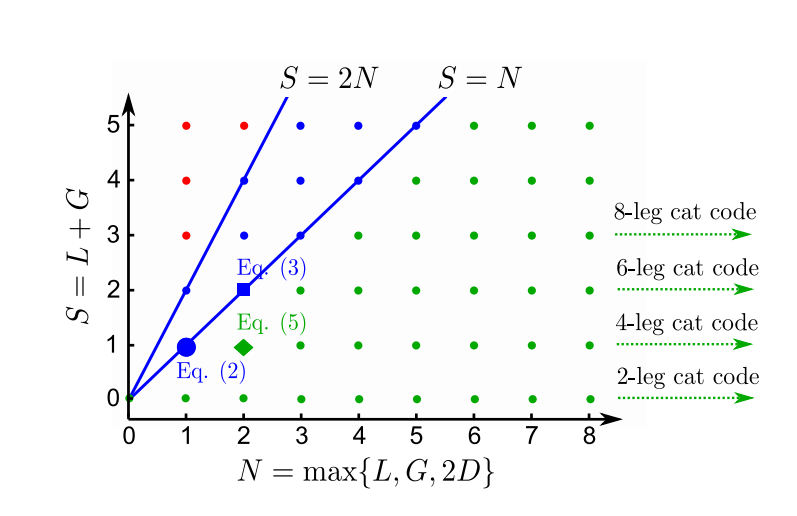
\includegraphics[width=0.5\linewidth,keepaspectratio]{Screenshot (958).png}	
\caption{Figure from \cite{michael2016new} comparing binomial codes to cat codes. Observe that, in principle, unlimited dephasing errors can be tolerated by cat codes.}
\end{figure}

\subsection{Performance Comparisons}
\label{sec:perf}


In their work \cite{albert2017performance}, Albert et al. introduce "channel fidelity", denoted as $F_\mathcal{E}$, as a practically feasible measure to assess the efficacy of single-mode bosonic code protection. The rationale behind this lies in the fact that the noise model operators might lack well-behaved properties, whereas optimal recovery for each code can be conveniently computed by employing a semi-definite program when channel fidelity is considered. Furthermore, if we assume that our noise is entirely characterized by the lossy bosonic channel (meaning perfect encoding, recovery, and decoding), then channel fidelity essentially quantifies the resilience of entanglement in the presence of the noisy bosonic channel. More specifically, it measures the degree of overlap between the initial state and the final state, with the initial state being an entangled Bell state, while only the first qubit is subjected to the influence of the noise channel.

\begin{figure}[ht]
\label{fig:perf}
\centering
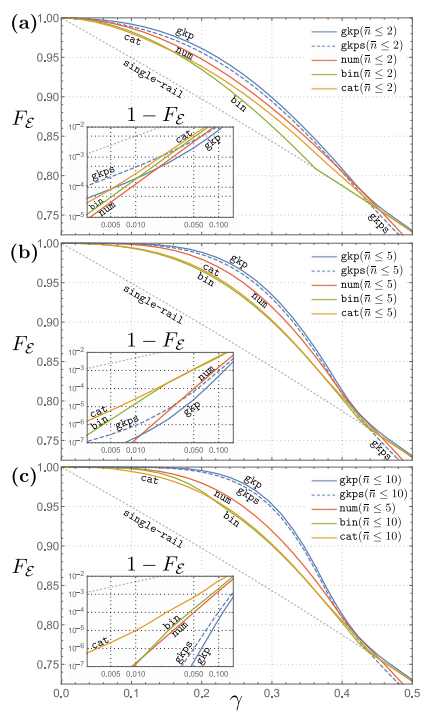
\includegraphics[width=0.5\linewidth,keepaspectratio]{Screenshot (960).png}	
\end{figure}


Figure \ref{fig:perf} provides an overview of the performance evaluation of the optimal code from each code family (determined through solving the semi-definite program), under the constraint of mean photon number, while varying the loss rate $\gamma$ (\ref{eq:gamma}).

The numerical findings demonstrate that codes designed to effectively counter predominant errors at low $\gamma$ might not necessarily translate into equally effective performance at higher $\gamma$ values. In our specific case, both cat and binomial codes ensure precise protection against initial loss errors by maintaining an adequate spacing, denoted as $S$, between Fock states, as previously described. Both cat and binomial codes offer the flexibility to increase $S$ arbitrarily, while gkp codes exhibit $S \in \{0, 1\}$ \cite{albert2017performance}, contingent on whether their lattice is displaced from the origin or not. Nonetheless, the gkp strategy of approximately suppressing all errors appears to yield the most promising results.

In a related vein, Noh et al. establish in their paper \cite{noh2018improved} that GKP codes achieve the quantum capacity of Gaussian loss channels, attaining this capacity up to a constant gap relative to an upper bound of the quantum capacity.

\subsection{Multi-Mode Extensions}

In this part, I aim to provide a concise overview of recent findings derived from these basic single-mode codes. The goal is to develop codes that can be practically implemented in the near future and offer comparable or even better error-correction abilities.

\subsubsection{Pair-Cat Codes}\label{sec:multi-cat}

The pair-cat codes introduced in \cite{albert2018multimode} by Albert et al. incorporate an extra mode not necessarily to enhance error-correction capabilities compared to traditional cat codes (although this becomes plausible with more than two modes), but rather to progress towards achievable physical implementation. This approach notably reduces the level of non-linearity required for realization.

The inherent uncorrectable error in this code is $\hat{a}\hat{b}$, where $\hat{a}$ and $\hat{b}$ represent loss operators acting on the first and second modes, respectively. Consequently, this replaces the uncorrectable error $\hat{a}^2$ in the case of single-mode cat codes, resulting in similar quality code subspaces.

Moreover, this method permits the simultaneous utilization of discrete quantum error correction (QEC) techniques (such as non-demolition measurement of error syndromes and dynamic control) and continuous QEC techniques. This parallel application is unfeasible in the context of single-mode scenarios using existing techniques.

To elaborate, recall that with cat codes, continuous "pumping" can suppress dephasing, and discrete photon loss recording can guard against losses. However, attempting both simultaneously is currently unattainable \cite{albert2018multimode}. This limitation is linked to the fact that the entangling gate for measurement is generated through a cross-Kerr interaction, which only commutes with the single-mode jump operator $J_1 \sim \hat{a}^4$ (as seen in equation \ref{eq:single-jump}) at discrete time intervals. Consequently, the dissipation due to $J$ must be halted during measurement. Interestingly, the pair-cat code's ability to utilize photon number differences, rather than parity, as syndromes permits fine-tuning of the parameters of the two-mode cross-Kerr interaction to commute with the pair-cat jump operator $J_2 \sim \hat{a}^2\hat{b}^2$.

Furthermore, Albert et al. propose a continuous error correction scheme against loss for the pair-cat codes using \textbf{Superconducting Nonlinear Asymmetric Inductive eLements (SNAILs)}\cite{frattini20173}. These require a lower-order non-linearity than the array of Josephson junctions required for continuous error correction against photon loss in the single-mode case.

Finally, we observe that $J_2$ spreads out the quartic stabilizing nonlinearity across two modes. This provides the advantage of requiring less photons per mode to have a comparable protection against dephasing and so a slightly lower probability of the leading uncorrectable loss error. Figure \ref{fig:cat} summarizes differences between the codes.

\begin{figure}[h]
\label{fig:cat}
\centering
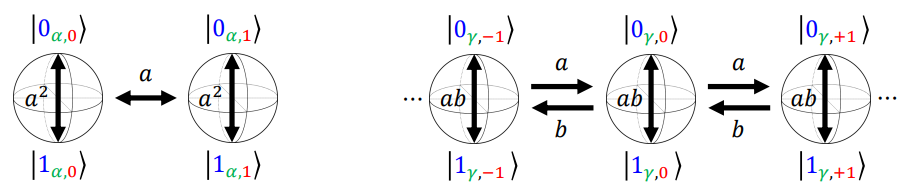
\includegraphics[width=\linewidth,keepaspectratio]{Screenshot (956).png}	
\caption{Figure from \cite{albert2018multimode} comparing single-mode cat codes to pair-cat codes}
\end{figure}

\subsubsection{$\chi^{(2)}$ Binomial Codes}
\label{sec:multi-binom}

The drive to develop new codes, such as pair-cat codes, stems from the fact that the universal gate set of single-mode cat codes relies on induced four-wave mixing interactions in Josephson junctions, which are significantly stronger than optical four-wave mixing in Kerr media. Thus, $\chi^{(2)}$ codes, encompassing a broader scope than the $\chi^{(2)}$ binomial codes we're focusing on here, aim to advance quantum computation by exclusively employing $\chi^{(2)}$ interactions for coherent photon conversion, alongside linear-optics transformations \cite{niu2018hardware}. This is because $\chi^{(2)}$ is a lower-order nonlinearity, potentially stronger than four-wave mixing.

To construct these codes, Niu et al. establish a symmetry-operator framework that harnesses the symmetry inherent in the physical subspace supporting logical codewords, as well as the symmetry of the measurable syndromes. This framework demonstrates that the $\chi^{(2)}$ binomial code represents the first Fock-basis bosonic quantum error correcting code capable of rectifying $N$ photon-loss errors using $O(N)$ photons for encoding. In contrast, all previously discussed codes necessitate encoding with $O(N^2)$ photons to correct $N$ photon-loss errors. However, this new code involves the utilization of channel-monitoring resources, unlike the other examined codes, which are employed to determine the number of photons lost or gained. This emphasizes the significance of channel monitoring for its potential to enhance error-correction capabilities.

Next, let's delve into the concept of "symmetry operators." We begin by considering an $N$-pump-photon 3-mode subspace $\mathcal{H}_N$. Within this subspace, all states $\ket{\psi} = \sum_{n=0}^N c_n \ket{n, n, N-n} \in \mathcal{H}_N$ adhere to the following relations:

\begin{align}
\begin{split}
	(\hat{n}_s + \hat{n}_p) \ket{\psi} &= N\ket{\psi} \\
	(\hat{n}_i + \hat{n}_p) \ket{\psi} &= N\ket{\psi} \\
	(\hat{n}_s - \hat{n}_i) \ket{\psi} &= 0\ket{\psi}
\end{split}
\end{align}

Here, $\hat{n}_k \equiv \hat{a}_k^\dag\hat{a}_k$ for each of the three modes, denoted as $k = s, i, p$. Consequently, the photon number parity vector can be expressed as:

\begin{align*}
P &= [\hat{n}_s + \hat{n}_i, \hat{n}_s + \hat{n}_p, \hat{n_i + n_p}  ] \mod 2\\
&= [2N, N, N] \mod 2
\end{align*}

is constant and is maintained for all $\ket{\psi}$. Drawing inspiration from this observation, we define symmetry operators:

\begin{align*}
\hat{Z}_{s, p}^{(N + 1)} = \exp(i 2 \pi / (N+1))	\hat{Z}_{s}^{(N + 1)} \otimes \hat{Z}_{p}^{(N + 1)} \\
\hat{Z}_{s, p}^{(N + 1)} = \exp(i 2 \pi / (N+1))	\hat{Z}_{s}^{(N + 1)} \otimes \hat{Z}_{p}^{(N + 1)}
\end{align*}

Here,

\begin{align*}
\hat{Z}_{k}^{(N + 1)} \equiv \sum_{n=0}^{N}\exp(i 2 \pi n / (N+1))	\ket{n}_k \bra{n}_k
\end{align*}

where $\ket{n}_k, n \in 0, 1, \cdots, N$ represents an $n$-photon Fock state of mode $k$ (where $k = s, i, p$).

To redundantly encode a lower-dimensional logical basis into a higher-dimensional physical basis, additional symmetry operators are required to stabilize the logical state. Specifically, within the code's physical subspace, only the eigenstates of all symmetry operators in the provided set with a unity eigenvalue are chosen as logical-basis states.

In the context of the $\chi^{(2)}$ binomial code, the physical-subspace symmetry characterized by $\{ \hat{Z}_{s, p}^{(2N)}, \hat{Z}_{s, p}^{(2N)}\}$ as defined above is enforced to confine logical basis states to the subspace $\mathcal{H}_N$. Furthermore, to leverage binomial symmetry that safeguards the code subspace against distortion from photon loss or gain errors, an additional symmetry is introduced involving the conjugation of the photon-number inversion operator with the pseudo-beam-splitter operator. For a more detailed understanding of this process, the original source \cite{niu2018hardware} is recommended.

What is crucial to highlight here is that this symmetry-operator framework establishes a systematic methodology for discovering novel quantum error correcting codes aligned with available measurement schemes and choices of physical subspace.

For instance, Niu et al. demonstrate that by completing the set of symmetry operators, the simplest scenario yields logical states:

\begin{align*}
	\ket{B_{\uparrow}} &\sim \ket{0, 0, 3} + \sqrt{3}\ket{2, 2, 1}\\
	\ket{B_{\downarrow}} &\sim \ket{3, 3, 0} + \sqrt{3}\ket{1, 1, 2}
\end{align*}

It can be verified using (\ref{eq:k-l}) that this code is resilient against up to second-order loss or gain, as well as first-order dephasing across all modes.

\subsubsection{Comparisons}

Let's proceed to compare the two multi-mode codes discussed above.

One fundamental distinction lies in the composition of pair-cat codes, which encompass infinite superpositions of Fock states, whereas $\chi^{(2)}$ codes are characterized by finite dimensions. Consequently, $\chi^{(2)}$ codes can only tolerate the loss of a finite number of photons, whereas pair-cat codes hold a non-zero, albeit exponentially diminishing, probability of experiencing the loss of any arbitrary number of photons.

It was previously noted that $\chi^{(2)}$ binomial codes can rectify more than one loss if the total count of lost photons is known (achieved through channel monitoring). On the other hand, generalized pair-cat codes can incorporate a concept of "spacing" denoted as $S$ (details can be found in Section V of \cite{albert2018multimode}), enabling the mitigation of up to $S$ loss errors in each mode solely through the information gleaned from error syndromes. Moreover, it has been revealed that pair-cat codes with a spacing of $S=0$ possess the ability to detect all loss and gain errors, even when considering three or more modes \cite{albert2018multimode}. This capability is beyond the reach of $\chi^{(2)}$ codes.

Nevertheless, in terms of error correction, the two-mode $\chi^{(2)}$ binomial codes can precisely rectify dephasing errors $n^l$, where $l \leq N$, whereas pair-cat codes offer approximate dephasing error correction.

\section{Conclusion}

\subsection{Importance of Bosonic Systems}

There are many potential advantages to bosonic systems. A clear one is that with each added qubit, several new decoherence channels are added, and this multiplies the number of possible errors and requires measuring more error syndromes. Therefore, it may be simpler to add physical degrees of freedom using bosonic continuous variable systems. Practically, too, it still seems extremely challenging to build a register of more than on the order of 10 qubits. Overall, then, bosonic systems may have strong use improving lifetimes of quantum memories.

Past quantum memory, bosonic mode quantum error correction is also useful for quantum teleportation and quantum communication \cite{michael2016new}, which consists of quantum state transfer and generation of high-fidelity entangled pairs of quantum bits between two distant nodes in a quantum network. In \cite{michael2016new} Michael et al. consider a 'pitch-and-catch' scenario for quantum state transfer which can be used for quantum repeaters. They show that simple bosonic codes can greatly increase the fidelity of quantum communication and remote entanglement between hardware modules by being utilized to protect errors from this protocol.

\subsection{Future Developments}

Significant advancements remain imperative to comprehensively assess the performance of bosonic error-correcting codes. It is crucial to recall the stringent assumptions made during the comparison of single-mode codes in Section \ref{sec:perf}: the perfection of encoding, recovery, and decoding processes, along with the grouping of codes based on mean photon occupation number. Furthermore, this performance analysis can be extended to various other multi-mode codes, and an intriguing avenue involves the expansion of this analysis to two modes. This extension could unveil the potential performance of pair-cat codes and $\chi^{(2)}$ binomial codes against photon loss, presenting a valuable exploration.

Moreover, the framework of symmetry operators, as described, furnishes a systematic approach for constructing bosonic QEC codes by leveraging the characteristics of the underlying system dynamics. This framework not only offers a smooth transition from qubit-basis three-mode encoding to qudit-basis multi-mode encoding but also holds promise for future endeavors that tap into this formalism.

Furthermore, $\chi^{(2)}$ binomial codes exhibit particular promise due to their efficient utilization of photon numbers (with an $O(N)$ dependence to rectify $N$ photon loss). However, these codes require "channel monitoring" to discern the number of loss errors at each time step. Thus, the efficient execution of this monitoring within the hardware emerges as a crucial prerequisite for the viability of these codes.

Nevertheless, the ultimate challenge lies in establishing hardware that is adept at efficiently carrying out these error correction procedures. The breakthrough achievement of achieving high-fidelity quantum non-demolition measurements of photon number parity, as demonstrated in \cite{sun2014tracking}, is noteworthy. The transition from single-mode codes like cat codes, which relied on microwave cavities coupled to Josephson junctions, to multi-mode codes represents a pivotal shift. Multi-mode codes leverage lower-order nonlinearities, potentially amendable by near-term realizable reservoir-engineered microwave cavities \cite{albert2018multimode} or facilitated through linear optics and $\chi^{(2)}$ interactions, thereby addressing the hardware challenge more effectively. The ongoing progress in this direction is indeed promising.

\nocite{*}
\newpage
\centering
\bibliography{qec_final_project.bib}
\bibliographystyle{amsplain}

\end{document}